\begin{figure*}[ht!]
\begin{center}
\vspace{-10pt}
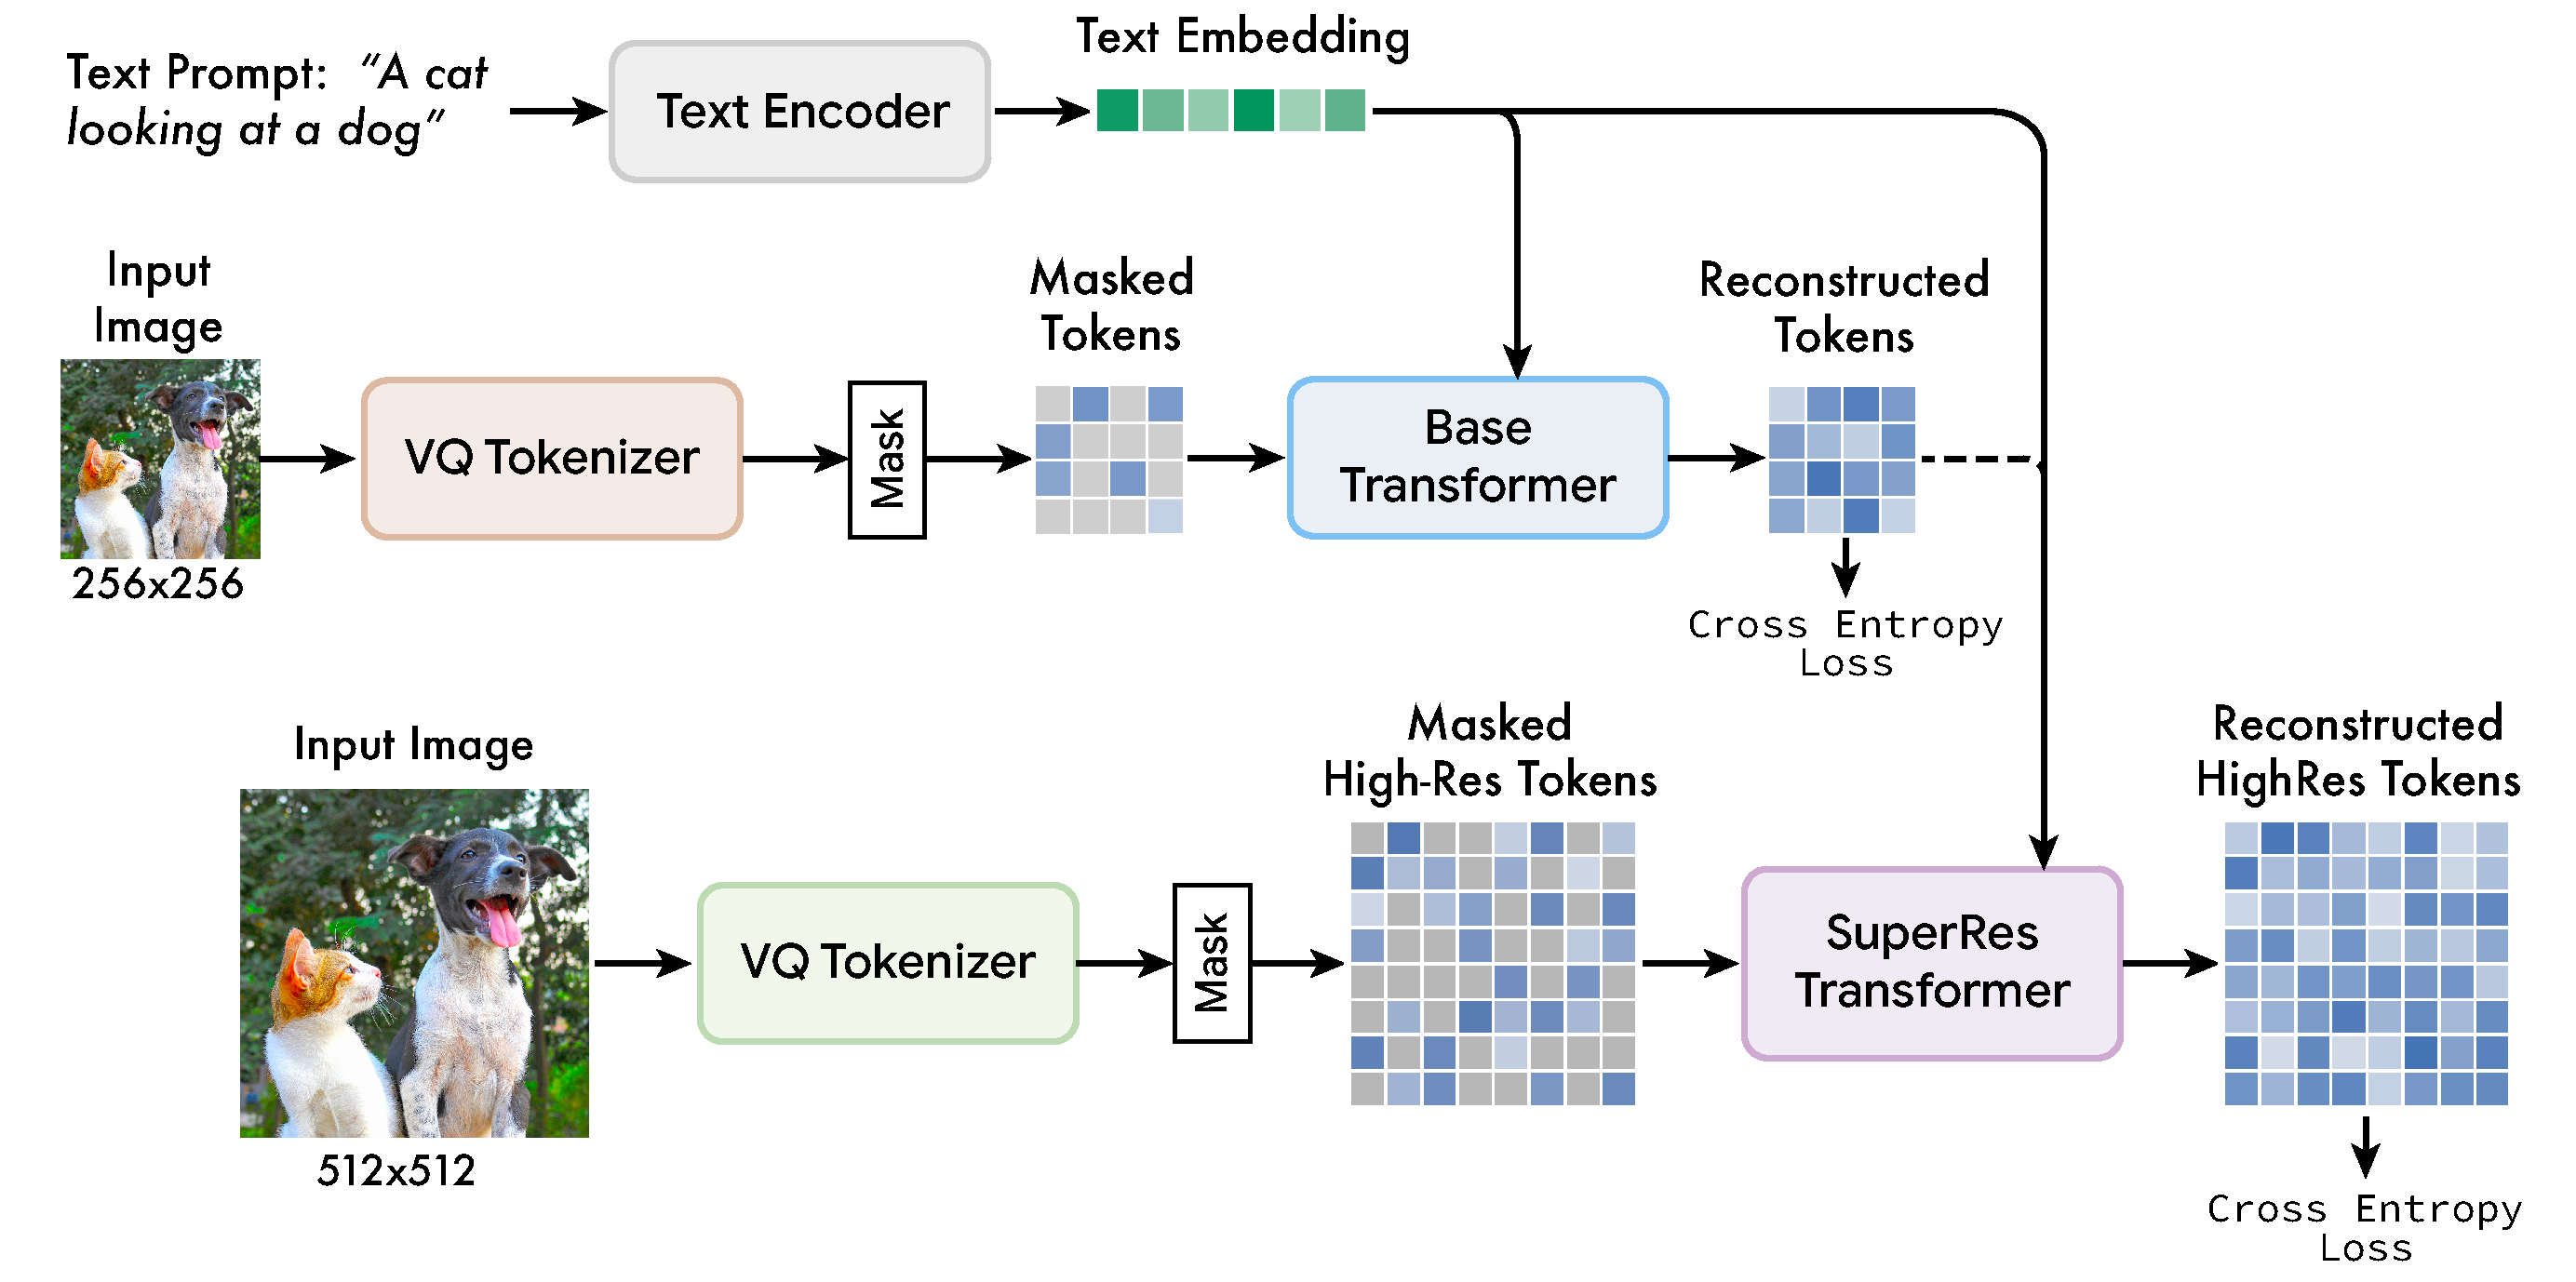
\includegraphics[width=.85\textwidth]{figs/pipeline_v4}
\end{center}
\vspace{-15pt}
\caption{\small \name~Framework: We show the training pipeline for our model, with the T5-XXL pre-trained text encoder, base model and super-resolution model depicted on the three rows. The text encoder generates a text embedding that is used for cross-attention with image tokens for both base and super-res Transformer layers. The base model uses a VQ Tokenizer that is pre-trained on lower resolution ($\lowres\times\lowres$) images and generates a $16\times16$ latent space of tokens. This sequence is masked at a variable rate per sample and then the cross-entropy loss learns to predict the masked image tokens. Once the base model is trained, the reconstructed lower-resolution tokens and text tokens are passed into the super-res model that then learns to predict masked tokens at a higher resolution. }

\vspace{-10pt}
\label{fig:model}
\end{figure*}